\documentclass[main.tex]{subfiles} % Subfile-Class


% ============================================================================== %
%                            Subfile document                                    %
% ============================================================================== %

\begin{document}

% Template

\subsubsection{Steuerungstopologie und Gesamtübersicht}~\label{sec:Gesamtuebersicht_Elektro}

Abbildung~\ref{fig:Gesamtuebersicht_vereinfacht} zeigt das Elektrokonzept in
einem kleinen Detaillierungsgrad. Ziel ist es, im Sinne der Gewaltenteilung
jede Steuerungseinheit für sich abgeschlossen zu betrachten. So kann sowohl die
Zuständigkeit der beiden Elektronikentwickler gut aufgeteilt werden, als auch
Schnittstellen zwischen Funktionseinheiten sehr eindeutig benannt werden.

\begin{figure}[H]
      \centering
      \includegraphics[width = 1\linewidth]{fig_Steuerungstopologie_Gesamtuebersicht/Vereinfacht.pdf}
      \caption{Vereinfachte Gesamtübersicht Elektronikkonzept}~\label{fig:Gesamtuebersicht_vereinfacht}
\end{figure}

Anhang~\ref{appendix:Blockschaltbild_Elektrokonzept} zeigt die Gesamtübersicht
der Steuerung zum Zeitpunkt von PREN1 nochmals in einer höheren Detaillierung.

\subsubsection*{Die verschiedenen Funktionsgruppen und ihre PCBs}
Es werden total die 4 folgenden Funktionsgruppen unterschieden:

\begin{description}
      \item[Raspberry HAT] Dieser PCB hat die Aufgabe, die nötige Peripherie für den
            Raspberry Pi zur Verfügung zu stellen. Dies beinhaltet die Anbindung
            verschiedener Taster an die entsprechenden GPIOs sowie eine
            Spannungsversorgung. Der Raspberry Pi soll ausserdem über einen Summer Signale
            wie das Erreichen des Zielpunktes signalisieren können. Weiter wird sein
            UART-Kanal für die Kommunikation aufbereitet.
      \item[Motion Controller] Dieser PCB bietet die Schnittstelle aller Steuereinheiten zu
            den Antrieben. Via UART werden diesem PCB Steuerkommandos wie 'fahren mit
            Geschwindigkeit \textit{xxx}', 'Fahrzeug um \textit{xxx°} drehen', 'Hindernis
            erkannt: Anhalten und warten' und viele weitere mitgeteilt. Er selbst
            beinhaltet Hardware zum Auszählen der Encoder sowie des Gyroskops und noch
            einige digitale Ein-/Ausgänge und Reserve-Sensorschnittstellen.
      \item[Grip Controller] Dieser PCB steuert, wie der Name erahnen lässt, alles rund um
            das Greifen und um den Umgang mit Hindernissen. Er erkennt das Hindernis und
            kann dem Motion Controller via UART Kommandos erteilen, wie das Anhalten oder
            dass das Fahrzeug gedreht werden soll.
      \item[Power Board] Das Power Board bietet die Spannungsaufbereitung für den Roboter.
            Hier werden aus den 14.4V Batteriespannung 12V Boardnetzspannung eingeregelt.
            Weiter wird die Batterie überwacht und bei drohender Unterspannung getrennt.
            Ausbalanciert wird eben diese Batterie über das externe Ladegerät. Wird ein
            14...18V Netzteil an diesem Board angeschlossen, wird die Batterie vom Fahrzeug
            getrennt, was Einricht- und Entwicklungsarbeiten erlaubt, ohne dass dazu eine
            Batterie benötigt wird.
\end{description}

Zum Stand von PREN1 wäre der Motion Controller grundsätzlich in der Lage, die
Aufgabe des Greifers ebenfalls zu übernehmen. Wenn sich der noch nicht
abgeschlossen getestete Greifmechanismus nicht eignet und mehr Motoren oder
Sensoren benötigt, hätte es auf diesem nicht mehr genug Schnittstellen für
Sensorik und Aktorik zur Verfügung. Daher wird mit dem separaten Grip
Controller geplant.

\subsubsection*{Kommunikationsschnittstellen}
Da Motoren, Schaltregler und andere Leistungselektronik auf engstem Raum mit
Kommunikations- und anderer empfindlicher Elektronik untergebracht werden müssen,
wird die UART-Kommunikation differentiell über eine RS422-Schnittstelle übertragen.
Die Kommandos und das Protokoll werden erst im Nachfolgemodul bei der Inbetriebnahme
dieser Leiterplatten endgültig definiert. Angedacht ist eine Kommunikation über
eine Kommandolänge von z.B. 64 Bit, in der eine Adresse, ein Kommando und zusätzlich
noch genügend Platz für zu übertragende Parameter definiert sind.  Abbildung~\ref{fig:Kommunikationsprotokoll}
zeigt den Aufbau einer solchen Nachricht.  Mögliche Parameter können eine Fahrzeuggeschwindigkeit,
ein Drehwinkel oder auch Fehlercodes sein, die an den Raspberry Pi zurückgesendet werden.

\begin{figure}[H]
      \centering
      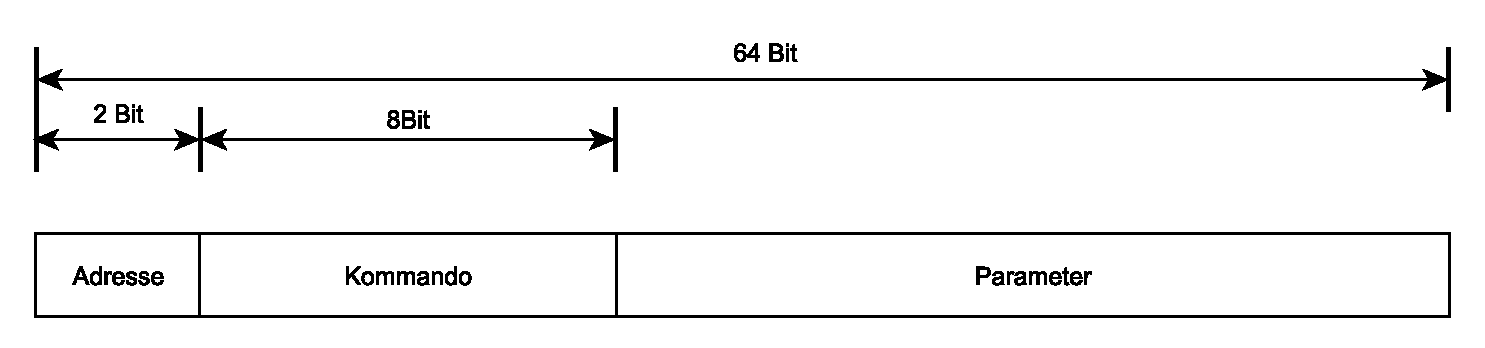
\includegraphics[width = 0.75\linewidth]{fig_Steuerungstopologie_Gesamtuebersicht/Kommunikationsprotokoll.pdf}
      \caption{Aufbau einer Nachricht}~\label{fig:Kommunikationsprotokoll}
\end{figure}

Die Adressvergabe, dargestellt in Abbildung~\ref{fig:Adressvergabe}, ist
vorgesehen, da der Raspberry Pi aufgrund der Kommunikationstopologie,
dargestellt im Blockschaltbild~\ref{fig:Gesamtuebersicht_vereinfacht},
grundsätzlich nicht in der Lage ist, direkt mit dem Greifcontroller zu
kommunizieren. Dies ist prinzipiell auch nicht notwendig. Um aber genau diesen
Fall abzudecken, sollten Adressen von $0 \dots 2$ (2-Bit) vergeben werden. So
kann eine einfache Punkt-zu-Punkt-Übertragung ausreichen, um die drei
Steuerungen miteinander kommunizieren zu lassen.

\begin{figure}[H]
      \centering
      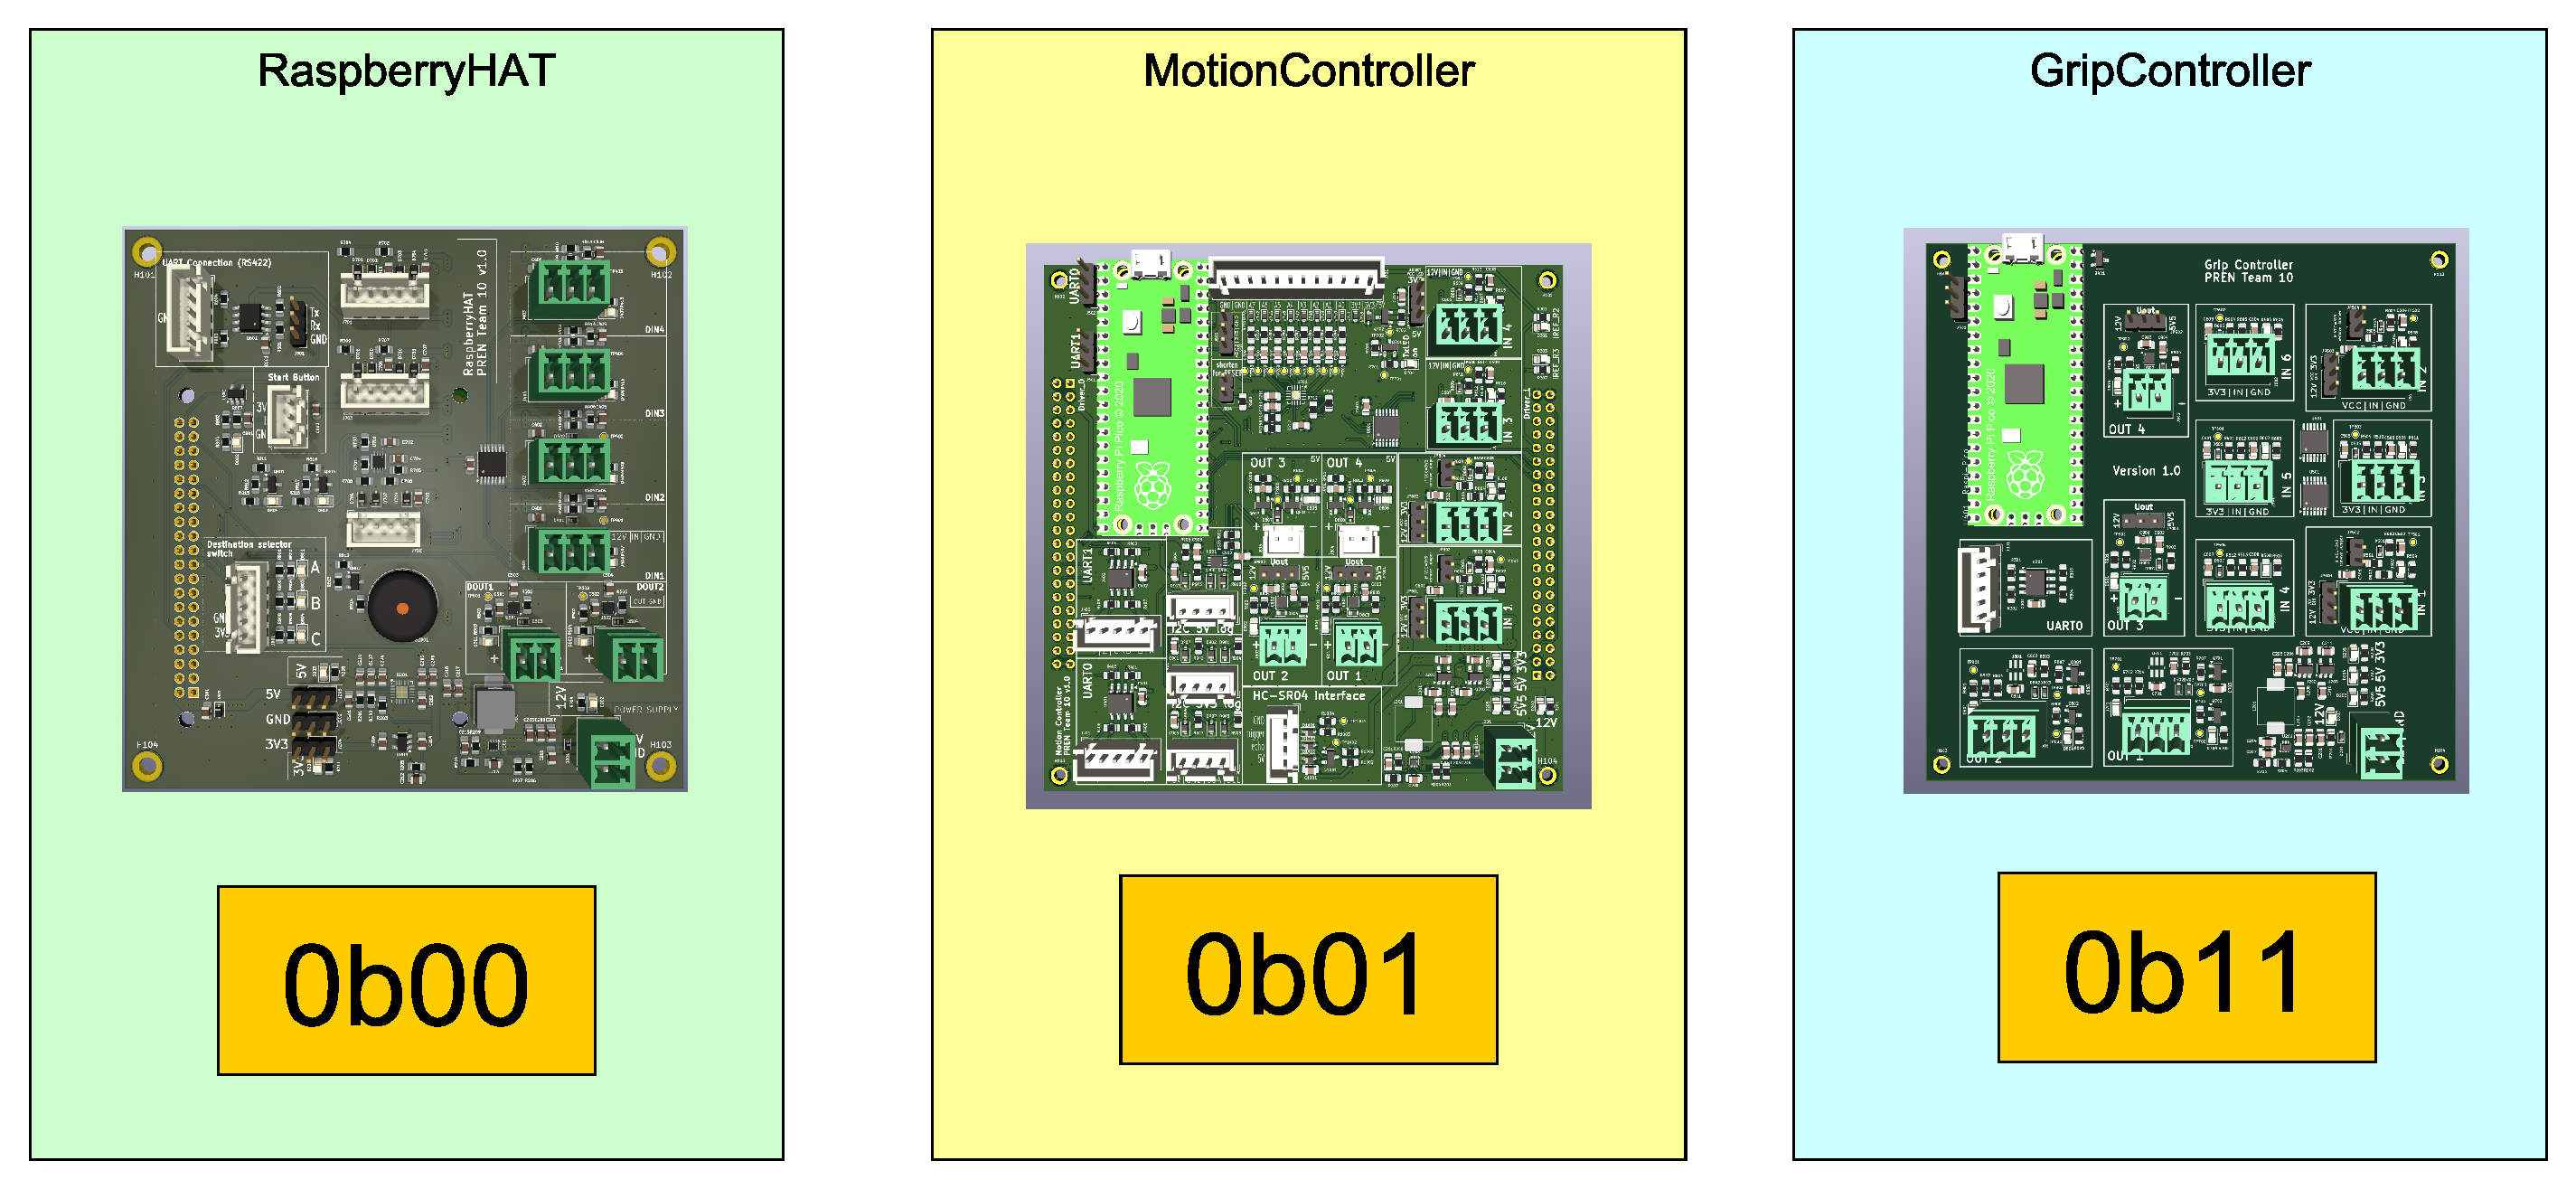
\includegraphics[width = 0.75\linewidth]{fig_Steuerungstopologie_Gesamtuebersicht/Adressvergabe.pdf}
      \caption{Vergebene Adressen der Prints}~\label{fig:Adressvergabe}
\end{figure}

\subsubsection*{Bordnetz}
Auf dieses wird in der Sektion~\label{sec:Boardnetz} im Detail eingegangen. Kurz ausgedrückt
besitzt jedes Board eine eigene Spannungswandlung von 12V auf 5V respektive 3.3V, welche vom
Power Board zur Verfügung gestellt werden.

\end{document}
